\documentclass[12pt,a4paperS]{report}
\usepackage[italian]{babel}
\usepackage[utf8]{inputenc}
\usepackage{graphicx}
\usepackage{natbib}
\usepackage{float}
\usepackage{hyperref}

\graphicspath{ {./img/} }

\begin{document}
	\begin{titlepage}
		\begin{center}
			
			\Large
			\textbf{Progetto Tecnologie Web 2023}
			
			\vspace{0.5cm}
			
			Documentazione del progetto sviluppato per il corso di Tecnologie Web
			
			\vspace{0.5cm}
			
			Anno scolastico: 2022/2023
			
			\vspace{1.5cm}
			
			\textbf{Gruppo 58}
			\vspace{0.5cm}
			
			\textbf{Antonio Colucci}
			
			\vspace{2.5cm}
			
			
\includegraphics[width=5.5cm]{logo_uni}
			
			\vspace{1.5cm}
			
			\Large
			Corso di Ingegneria Informatica e dell'Automazione presso l'Università Politecnica delle Marche
		\end{center}
	\end{titlepage}
	\tableofcontents
	\newpage
	
	\hypertarget{descrizione}{\chapter{Descrizione del sito}}
	\label{descrizione}
		\begin{normalsize}
			Il sito sviluppato è dedicato ad un'azienda di noleggio auto.
			L'azienda offre appunto servizi di noleggio di svariati modelli di auto suddivisi per categoria:
			\begin{itemize}
				\item Auto piccole: sono automobili compatte, ottime per l'utilizzo in città e per piccoli spostamenti;
				\item Auto medie: sono automobili non troppo grandi, che permettono un buon utilizzo cittadino, ma anche possibilità di spostamenti più lunghi;
				\item Auto grandi: sono automobili comode e con qualche accorgimento tecnologico in più. Sono ottime per affrontare lunghi spostamenti ed offrono maggiore spazio per i bagagli;
				\item SUV: sono auto grandi e alte, che permettono una visuale migliore alla guida ed un comfort di altissimo livello.
			\end{itemize}
			Il sito offre quattro livelli di utenza, suddivisi in base a diverse funzionalità:
			
			\section{Utente pubblico}
				Gli utenti pubblici posso accedere alle funzionalità base del sito, che sono comuni a tutti i livello di utenza.
				\newline
				Nel dettaglio essi possono: reperire informazioni sull'azienda e sulla sua posizione; reperire dettagli sui servizi offerti; ottenere maggiori informazioni consultando le FAQ; accedere al catalogo delle auto che l'azienda mette a disposizione per il noleggio; accedere al sito con le proprie credenziali, oppure effettuare la registrazione di un nuovo account.
				
			\section{Utente registrato (Cliente)}
				I clienti sono gli utenti che hanno effettuato la registrazione al sito, quindi possiedono un proprio account.
				\newline
				Oltre a poter usufruire di tutte le funzionalità di un utente pubblico (eccezione fatta per la registrazione di un nuovo account), i clienti possono: noleggiare un'automobile per un determinato periodo di tempo scelto in fase di noleggio; modificare i dati personali nella propria area riservata.
			
			\section{Membro dello staff aziendale}
				Quest'area è dedicata ai membri dello staff aziendale ovvero a tutti i dipendenti, i quali possono: accedere al catalogo auto per andare a modificare o eliminare le auto già presenti in catalogo; inserire una nuova auto, specificando tutti i dettagli e fornendo delle foto esterne; visualizzare un elenco delle auto noleggiate e dei rispettivi clienti, in un determinato mese scelto all'inizio.
			
			\section{Amministratore}
				L'amministratore dell'azienda può effettuare tutte le operazioni consentite agli utenti pubblici ed allo staff, inoltre può: gestire tutto lo staff (creazione, modifica ed eliminazione dei membri); cancellare gli utenti registrati; aggiornare le FAQ del sito; accedere ad un'area dove può ottenere, per l'anno corrente, il numero di auto noleggiate in base al mese scelto.
		\end{normalsize}
		
	\hypertarget{diagrammi}{\chapter{Diagrammi e schemi del Sito}}
	\label{diagrammi}
		\begin{normalsize}
			\section{Schemi dei link}
				Di seguito vengono riportati gli schemi dei link, divisi per livello di utenza, i quali forniscono una visione completa di tutti i collegamenti delle pagine del sito.
				\begin{figure}[H]
					\centering
					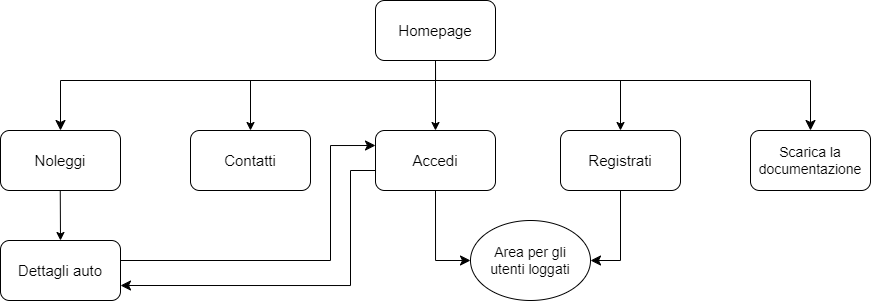
\includegraphics[width=1.15\textwidth, height=1.15\textheight, trim=100 0 0 0,keepaspectratio]{Grafici/Link_sez_pubblica.png}
					\newline
					\caption{Schema dei link della sezione pubblica}
				\end{figure}
				\begin{figure}[H]
					\centering
					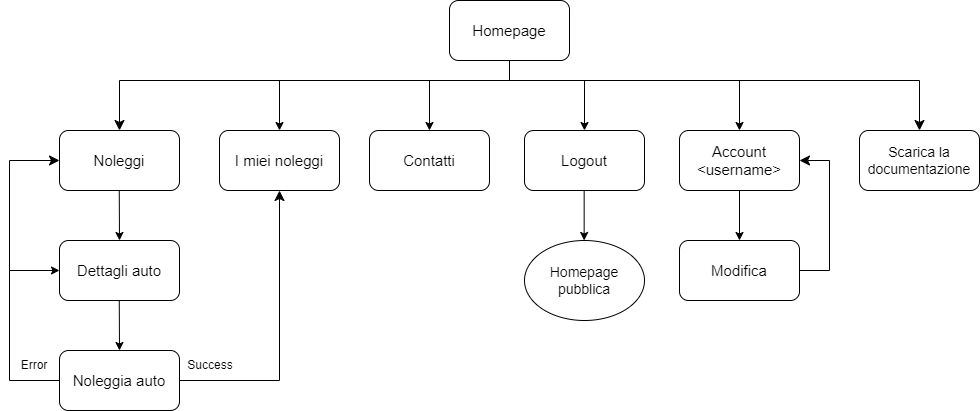
\includegraphics[width=1.15\textwidth, height=1.15\textheight, trim=100 0 0 0,keepaspectratio]{Grafici/Link_sez_clienti.png}
					\caption{Schema dei link della sezione clienti}
				\end{figure}
				\begin{figure}[H]
					\centering
					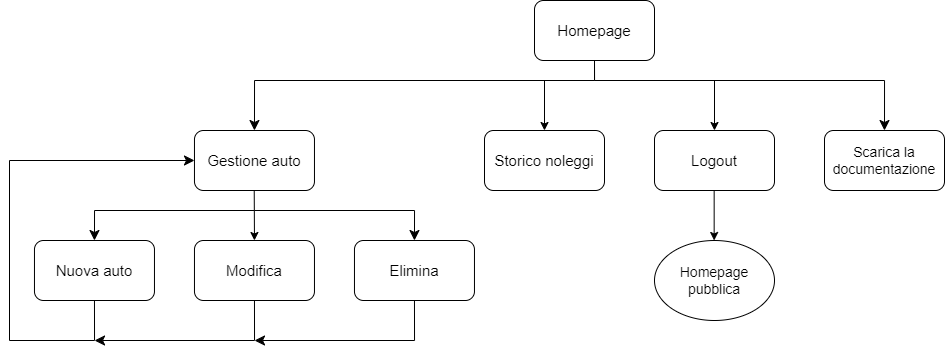
\includegraphics[width=1.15\textwidth, height=1.15\textheight, trim=100 0 0 0,keepaspectratio]{Grafici/Link_sez_staff.png}
					\newline
					\caption{Schema dei link della sezione staff}
				\end{figure}
				\begin{figure}[H]
					\centering
					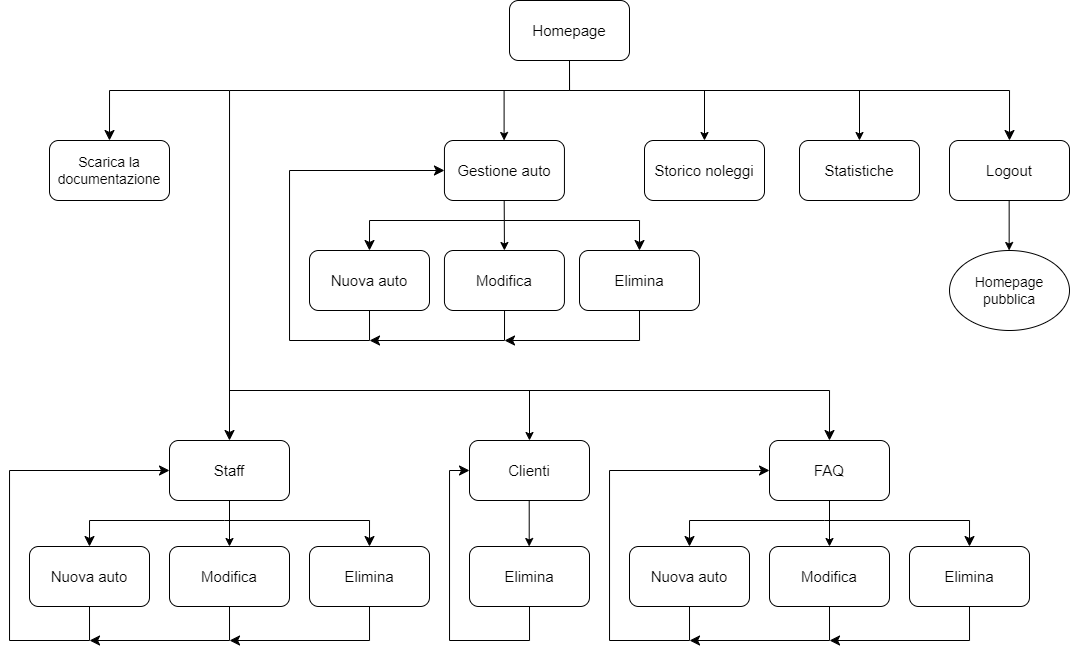
\includegraphics[width=1.15\textwidth, height=1.15\textheight, trim=100 0 0 0,keepaspectratio]{Grafici/Link_sez_admin.png}
					\caption{Schema dei link della sezione admin}
				\end{figure}
				
			\section{Database}
				Il database è composto da 4 tabelle: una dedicata alla categoria rappresentante un gruppo di auto; una dedicata alle auto; una per la FAQ; una per gli utenti.
				\newline
				Per quanto riguarda la relazione tra Auto e Categoria, ogni auto appartiene ad una ed una sola categoria, mentre ogni categoria può avere diverse automobili.
				\newline
				Parlando invece della relazione tra Auto ed Utente, ogni utente può noleggiare più auto, ma in periodi diversi, ed ugualmente un'auto può essere noleggiata da più utenti in periodi diversi.
				\subsection{Schema E-R}
					\begin{figure}[H]
						\centering
						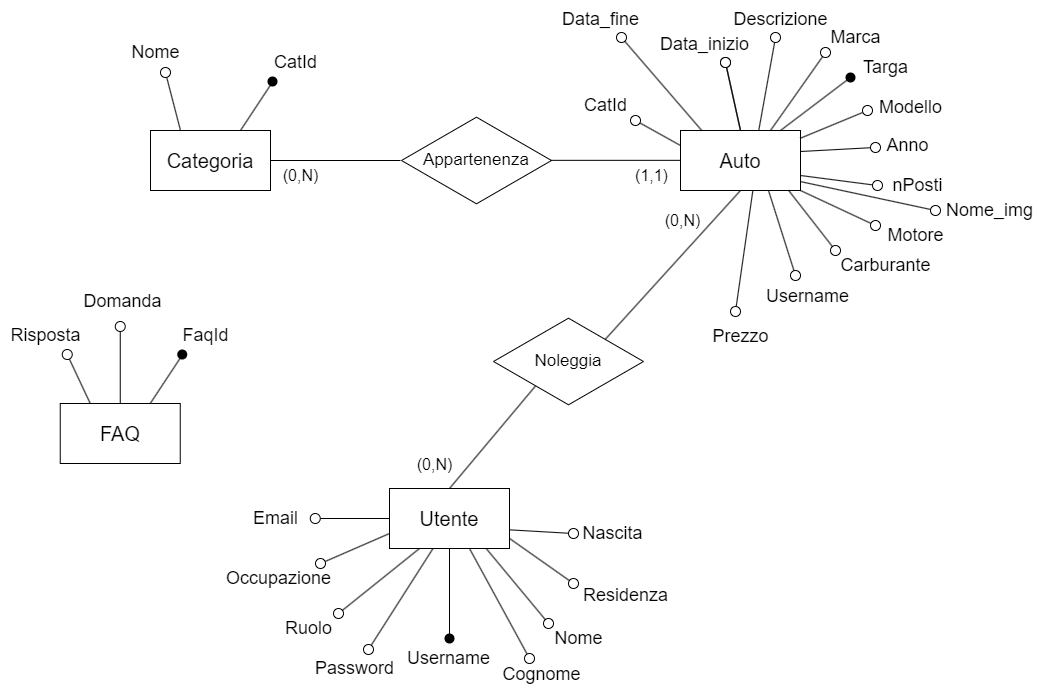
\includegraphics[width=1.15\textwidth, height=1.15\textheight, trim=100 0 0 0,keepaspectratio]{Grafici/Database.png}
						\newline
						\caption{Schema E-R del DB}
					\end{figure}
		\end{normalsize}
		
	\hypertarget{mockup}{\chapter{Mockup}}
	\label{mockup}
	\begin{normalsize}
		In questo capitolo verranno inserite tutte le immagini del mockup realizzato.
		
		\section{Sezione pubblica}
			Le immagini seguenti rappresentano tutte le pagine di cui si compone la sezione pubblica del sito.
			\subsection{Homepage}
				La homepage è la medesima sia per gli utenti registrati che non.
				\newline
				L'unica differenza si trova nella barra di navigazione, perchè gli utenti loggati avranno il pulsante per il logout e quello per accedere al proprio account, mentre gli utenti pubblici hanno i bottoni "Registrati" e "Accedi".
				\begin{figure}[H]
					\centering
					\includegraphics[width=0.95\textwidth, height=0.95\textheight, keepaspectratio]{Mockup/Homepage.png}
					\caption{Homepage pubblica}
				\end{figure}
				
			\subsection{Catalogo noleggi}
				Il catalogo delle auto è lo stesso sia per gli utenti registrati che non.
				\newline
				\begin{figure}[H]
					\centering
					\includegraphics[width=0.91\textwidth, height=0.91\textheight, keepaspectratio]{Mockup/Catalogo.png}
					\caption{Catalogo noleggi}
				\end{figure}
			
			\subsection{Dettagli auto selezionata}
				La pagina riguardante i dettagli dell'auto selezionata nel catalogo è la medesima sia per gli utenti registrati che non.
				\newline
				Ricordo che il noleggio effettivo dell'auto può essere eseguito solo dagli utenti registrati, infatti qualora un utente non registrato cliccasse sul tasto "Noleggia", verrebbe reindirizzato alla pagina di login.
				\newline
				\begin{figure}[H]
					\centering
					\includegraphics[width=0.82\textwidth, height=0.82\textheight, keepaspectratio]{Mockup/Dettagli_auto.png}
					\caption{Dettagli auto}
				\end{figure}
			
			\subsection{Contatti}
				La pagina riguardante i contatti dello sviluppatore è identica sia per gli utenti registrati che non.
				\begin{figure}[H]
					\centering
					\includegraphics[width=1\textwidth, height=1\textheight, keepaspectratio]{Mockup/Contatti.png}
					\caption{Contatti}
				\end{figure}
				
			
			\subsection{Login}
				\begin{figure}[H]
					\centering
					\includegraphics[width=1\textwidth, height=1\textheight, keepaspectratio]{Mockup/Login.png}
					\caption{Form per il login}
				\end{figure}
			
			\subsection{Registrazione}
				\begin{figure}[H]
					\centering
					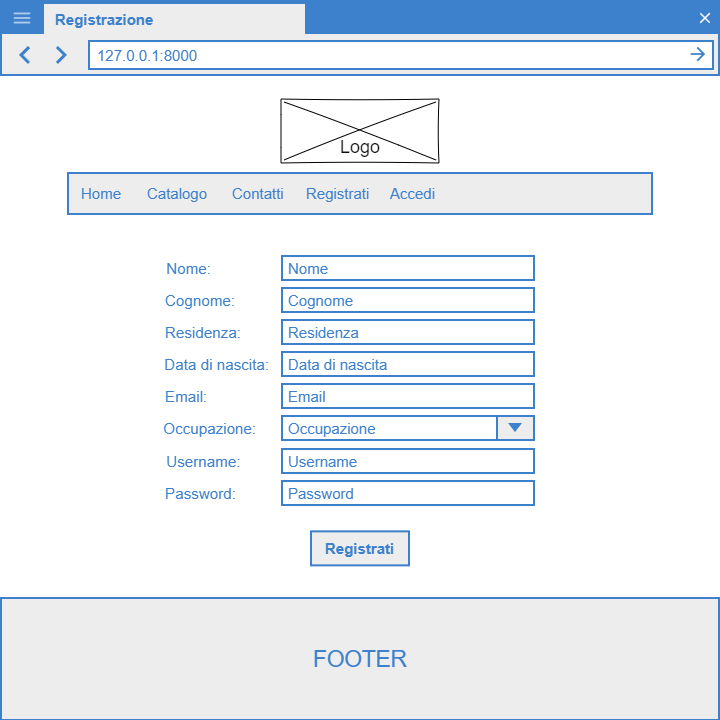
\includegraphics[width=1\textwidth, height=1\textheight, keepaspectratio]{Mockup/Registrazione.png}
					\caption{Form per la registrazione di un nuovo utente}
				\end{figure}
		
		\section{Sezione clienti}
			Le immagini seguenti rappresentano tutte le pagine di cui si compone la sezione riservata agli utenti registrati al sito.
			
			\subsection{I miei noleggi}
				\begin{figure}[H]
					\centering
					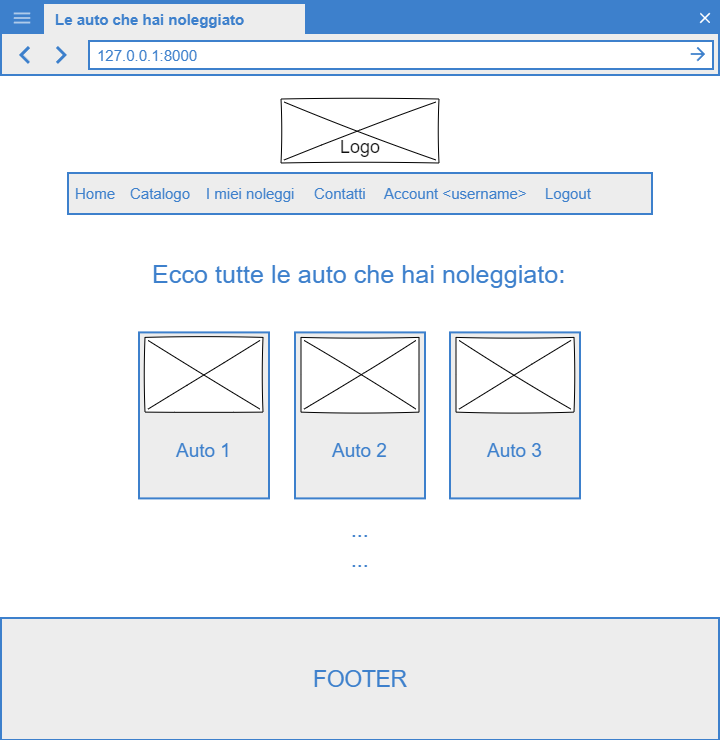
\includegraphics[width=1\textwidth, height=1\textheight, keepaspectratio]{Mockup/Storico_noleggi_utente.png}
					\caption{Storico delle auto noleggiate}
				\end{figure}
			
			\subsection{Area riservata}
				\begin{figure}[H]
					\centering
					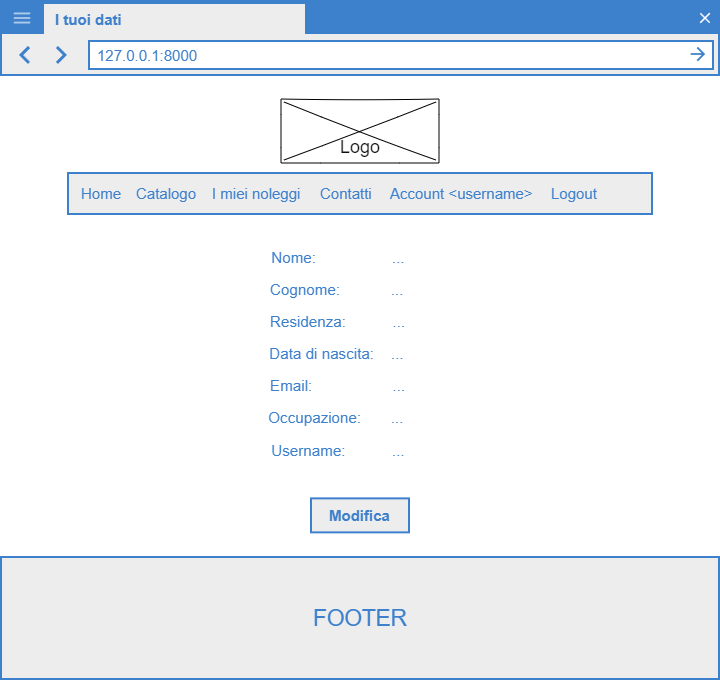
\includegraphics[width=1\textwidth, height=1\textheight, keepaspectratio]{Mockup/Area_riservata.png}
					\caption{Area riservata con i dati personali del cliente}
				\end{figure}
			
			\subsection{Modifica dati personali}
				\begin{figure}[H]
					\centering
					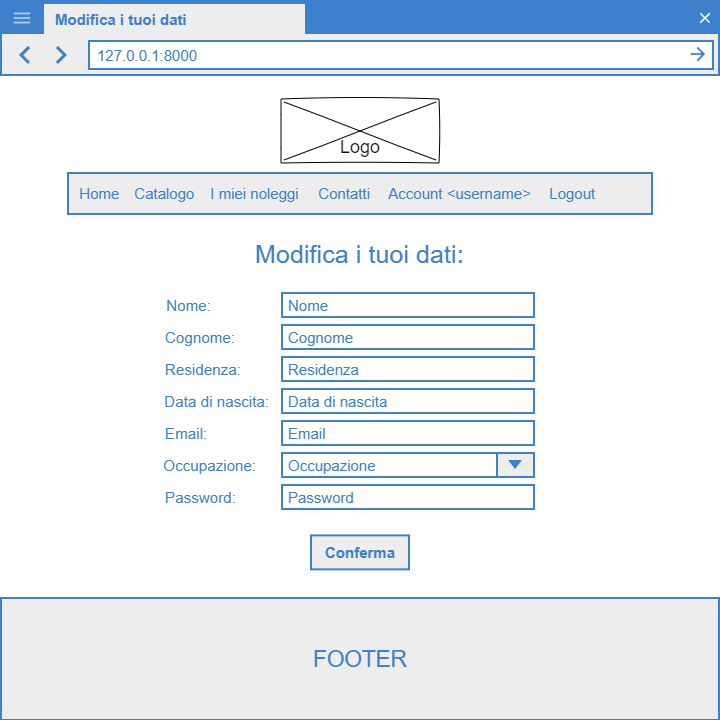
\includegraphics[width=1\textwidth, height=1\textheight, keepaspectratio]{Mockup/Modifica_dati.png}
					\caption{Form di modifica dei dati personali}
				\end{figure}
				
		\section{Sezione staff}
			Le immagini seguenti rappresentano tutte le pagine di cui si compone la sezione riservata ai membri dello staff.
			
			\subsection{Home staff}
				La homepage dello staff è identica a quella pubblica, con l'aggiunta di un saluto iniziale.
			
			\subsection{Gestione auto}
				Qui troviamo un'area dedicata alla gestione delle auto, ovvero permette l'inserimento, la modifica e l'eleminazione di una o più automobili.
				\newline
				Questa pagina è usata anche dall'admin.
				\begin{figure}[H]
					\centering
					\includegraphics[width=1\textwidth, height=1\textheight, keepaspectratio]{Mockup/Gestione_auto.png}
					\caption{Pagina per le gestione delle auto}
				\end{figure}
			
			\subsection{Nuova auto}
				Questa pagina è usata anche dall'admin.
				\begin{figure}[H]
					\centering
					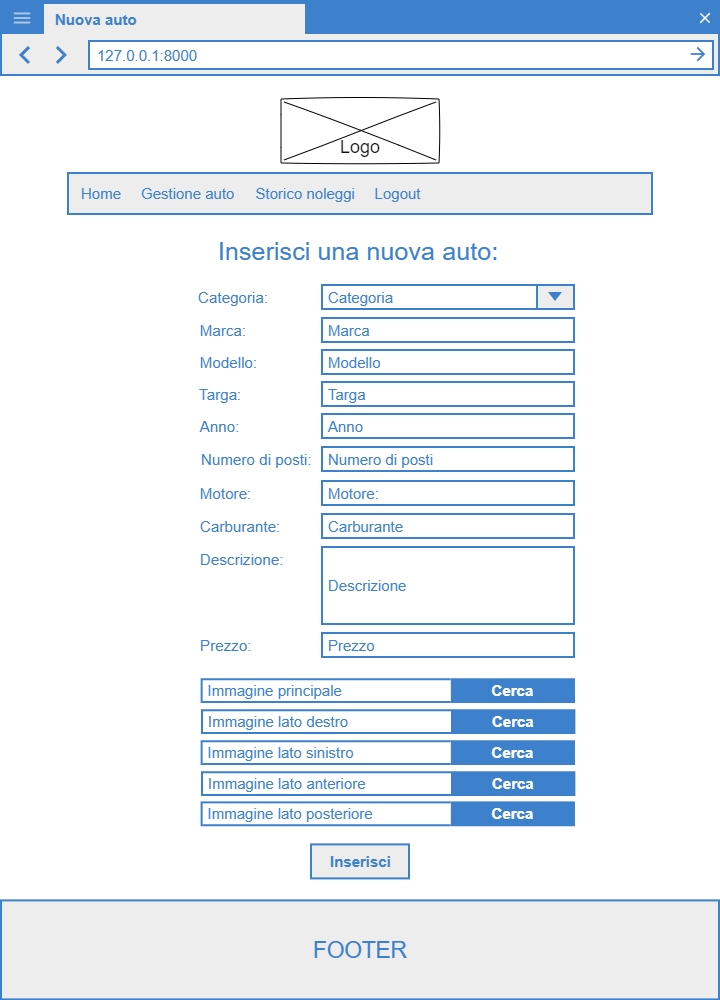
\includegraphics[width=0.85\textwidth, height=0.85\textheight, keepaspectratio]{Mockup/Nuova_auto.png}
					\caption{Form di inserimento di una nuova auto}
				\end{figure}
			
			\subsection{Modifica auto}
				La pagina dedicata alla modifica dei dati di un'auto selezionata è identica alla pagina per l'inserimeno di una nuova auto.
				\newline
				Questa pagina è usata anche dall'admin.
			
			\subsection{Storico dei noleggi}
				Lo staff sceglie un mese e potrà visualizzare l'elenco delle automobili noleggiate quel mese.
				\newline
				Questa pagina è usata anche dall'admin.
				\begin{figure}[H]
					\centering
					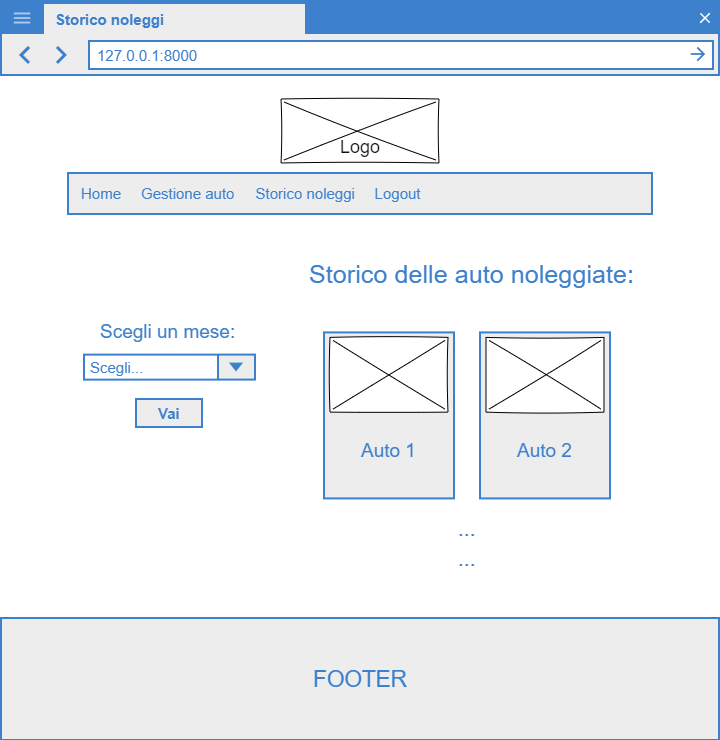
\includegraphics[width=0.88\textwidth, height=0.88\textheight, keepaspectratio]{Mockup/Storico_noleggi_staff.png}
					\caption{Storico dei noleggi di un dato mese}
				\end{figure}
				
		\section{Sezione admin}
			Le immagini seguenti rappresentano tutte le pagine di cui si compone la sezione riservata all'amministratore dell'azienda.
			
			\subsection{Home Admin}
				La homepage dell'admin è identica a quella pubblica, con l'aggiunta di un saluto iniziale.
			
			\subsection{Gestione Staff}
				*Immagine*
			
			\subsection{Inserimento membro staff}
				*Immagine*
			
			\subsection{Modifica dati membro staff}
				*Immagine*
			
			\subsection{Gestione Clienti}
				*Immagine*
		
			\subsection{Gestione FAQ}
				*Immagine*
			
			\subsection{Inserimento nuova FAQ}
				*Immagine*
			
			\subsection{Modifica FAQ}
				*Immagine*
			
			\subsection{Statistiche}
				*Immagine*
			
	\end{normalsize}
	
	\hypertarget{soluzioni}{\chapter{Soluzioni tecnologicamente interessanti}}
	\label{soluzioni}
	\begin{normalsize}
		contenuto...
	\end{normalsize}
\end{document}